Eine senkrechte Feder steht auf dem Boden. Legt man eine Kiste (\mKO) darauf, wird die Feder um \dxO\ zusammengedrückt, und die Kiste ruht. \DuSie{Rechne}{Rechnen Sie} mit \gO.

\begin{center}
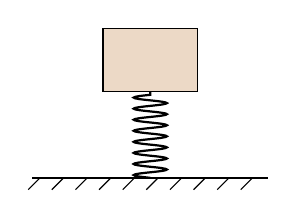
\begin{tikzpicture}
 \draw[thick] (-1.5,0) -- (1.5,0);
 \foreach \x in {-1.4,-1.1,...,1.4} \draw (\x,0) -- ++(-0.15,-0.15);
 \draw[thick, decorate, decoration={coil, aspect=0, segment length=4pt, amplitude=6pt}] (0,0) -- (0,1.1);
 \draw[thick] (-0.4,1.1) -- (0.4,1.1);
 \draw[fill=brown!30] (-0.6,1.1) rectangle (0.6,1.9);
\end{tikzpicture}
\end{center}

\begin{abcliste}
\abc
\DuSie{Zeichne}{Zeichnen Sie} die Kräfte auf die Kiste ein. In welche Richtung zeigt die Federkraft, und warum?

\abc
\DuSie{Berechne}{Berechnen Sie} die Federkonstante der Feder.

\abc
Nun hängt man dieselbe Kiste an dieselbe Feder, die an der Decke befestigt ist. Wie stark wird die Feder jetzt verformt, und in welche Richtung zeigt die Federkraft auf die Kiste?
\end{abcliste}
